\documentclass{article}

% if you need to pass options to natbib, use, e.g.:
%     \PassOptionsToPackage{numbers, compress}{natbib}
% before loading neurips_2018

% ready for submission
% \usepackage{neurips_2018}


% to compile a preprint version, e.g., for submission to arXiv, add add the
% [preprint] option:
%     \usepackage[preprint]{neurips_2018}

% to compile a camera-ready version, add the [final] option, e.g.:
\usepackage[final]{nips_2018}

% to avoid loading the natbib package, add option nonatbib:
%     \usepackage[nonatbib]{neurips_2018}

\usepackage[utf8]{inputenc} % allow utf-8 input
\usepackage[T1]{fontenc}    % use 8-bit T1 fonts
\usepackage{hyperref}       % hyperlinks
\usepackage{url}            % simple URL typesetting
\usepackage{booktabs}       % professional-quality tables
\usepackage{amsfonts}       % blackboard math symbols
\usepackage{nicefrac}       % compact symbols for 1/2, etc.
\usepackage{microtype}      % microtypography
\usepackage{bm}
\usepackage{amsmath}
\usepackage{amssymb}
\usepackage{amsthm}
\usepackage{graphicx}
\usepackage{bbold}
\title{3D Object Classification}

\author{
  Team members: Jiawei Chen, Linlin Li
}

\begin{document}

\maketitle
\section*{Abstract}
Convolutional Neural Networks (CNNs) have been used on 3D point clouds for object classification. However, due to the nature of the CNNs, classifiers, especially those CNN-based classifiers, are usually confused about objects that look alike. In this project, we propose a two-stage PointConv, a new method inspired by \textit{PointConv}, which aims to improve the performance in the classes with a similar appearance. Experiments were carried out using \textit{ModelNet40} to train and test the system.

\section{Introduction}

With the breakthroughs of self-driving devices and the potential in augmented reality applications, it is becoming increasingly important to develop methods to solve the tasks in 3D geometric data analysis, such as object classification, part recognition, and scene segmentation. However, unlike 2D images which consist of well-aligned points on an underlying grid, 3D geometric data such as meshes or point clouds are unordered and irregular. Therefore, it is impractical to directly apply methods in 2D image recognition into 3D space. 

To address this problem, a proposal has been made to either project 3D objects along with different directions into a 2D grid, or to quantize point clouds into a structured 3D grid, but both have limitations in terms of memory efficiency and resolution problems. In recent years, methods have been proposed allowing deep learning networks to process raw point clouds directly \cite{pointnet}, which significantly improved the efficiency and deep learning methods and gave rise a series of model applications in 3D space based on multiple layer perceptrons (MLPs), generative adversarial networks (GANs) and convolutional neural networks (CNNs).

\subsection{Motivation and importance of the problem}

After reviewing a considerable amount of literature in 3D object classification, we noticed that among the state-of-the-art designs, CNN and its variants enjoyed great popularity among researchers due to its capability of capturing neighborhood relationships instead of focusing only on individual points in the clouds. However, it is also CNN's heavy reliance on detecting combinations of features that is responsible for models' confusion on classifying objects that look alike, such as recognize a table against a desk.

Thus, in this project, we propose an approach to specifically address the problem in which CNN-based deep learning geometric models get confused over similar-looking 3D objects, by employing a two-stage 3D object classifier. We combined the confusing categories into a new class. The first stage focusing on classifying the original unconfusing categories plus the newly formed one, and the second stage is specifically trained to classify those easily-confusing shapes. Then we aggregated the results from two classifiers based on the theory of conditional probability.

\section{Related works}
Traditionally, researchers achieved object classification by handcrafting feature descriptors to capture the similarities between shapes. For example, Belongie et al.\cite{shapecontexts} attached a descriptor named the shape context to obtain the distribution of the remaining points to a reference point, which offered a globally discriminative characterization for classifying objects. Other similar handcrafted feature descriptors include the spin images from Johnson et al.\cite{spin}, the point feature histograms from Rusu et al.\cite{featurehist}, and the normal histograms from Tombari et al.\cite{normalhist}. However, efforts need to be taken in order to build these descriptors and their generability is often unsatisfactory in terms of applications to other object classification problems.

In recent years, due to the growing computational resources and the breakthrough results of CNN in 2D image recognition, researchers started to design data-driven deep learning architectures to extract feature information and thus recognize shapes in 3D automatically. However, unlike images that have pixels aligned neatly in an underlying grid, points of a 3D object (point clouds or meshes) are normally considered irregular. Thus, some preprocessing or transformations are needed if the same 2D architectures are to be applied to 3D geometric data.

One of the common methods is to project a point cloud into 2D spaces from different directions so that 2D CNNs could be applied to extract features, such as the methods proposed by Wu et al. \cite{modelnet} and Wei et al. \cite{dense}. Then some pooling layer is deployed in order to aggregate the information from different images of a shape, which would then be used for the classification tasks. This method has actually achieved great success and high accuracy on object classification with well-designed architectures, although it is hard to extend it into high-resolution cases or other tasks in 3D space such as scene segmentation. 

Alternatively, Maturana et al. \cite{voxnet} has proposed a method to quantize the 3D object into a structured 3D grid, named volumetric grid, in order to apply 3D CNNs. Wang et al. \cite{voxseg} then extended that into scene segmentation tasks. However, due to the sparsity of point clouds, the resulted grid is usually of unsatisfactory resolution and still needs demanding computational resources in the quantization process. Although some workarounds have been proposed by Klokov et al. \cite{kd} to address the resolution problem and Graham et al. \cite{sscn} to improve memory and speed, these solutions also incurred other limitations, which rendered the volumetric grid representation less ideal for 3D object tasks.

In recent years, some novel yet effective methods have been proposed to consume point clouds directly. Qi et al. \cite{pointnet} pioneered this area by employing a transformation network layer, some shared MLP layers, and max-pooling layers which covered the sparsity, permutation invariance, and transformation invariance of point clouds simultaneously. Then, the same group of researchers improved their network further by incorporating a hierarchical structure, making it easier to combine extracted features from different scales \cite{pointnetpp}. However, it is worth noticing that these methods work on individual points, and thus the local relationship for a point within its neighborhood is lost. In order to address this problem, researchers started to design variants of these two structures. Wang et al. \cite{dgcnn} proposed an edge convolutional operator, EdgeConv to generate edge features that can describe local neighborhood relationships and designed Dynamic Graph CNN (DGCNN) which is able to dynamically update the graph. Zhang et al. \cite{ldgcnn} then optimized the DGCNN structure by linking the hierarchical features from different dynamic graphs and designed Linked DGCNN. On the other hand, Wu et al. \cite{pointconv} proposed another convolutional operation, \textit{PointConv}, which is a memory-efficient density re-weighted convolution approach, allowing it to scale up to a lot of modern CNNs.

\section{Details of the project}
\subsection{Contribution of each member of the team}
\textbf{Jiawei Chen}, Master's in Statistical Science, Duke University.
\begin{itemize}
  \item[--] Literature review
  \item[--] Comparative analysis 
  \item[--] Implementation
  \item[--] Report writeup 
\end{itemize}

\textbf{Linlin Li}, Master's in Statistical Science, Duke University.
\begin{itemize}
  \item[--] Data preprocessing
  \item[--] Two-stage proposal
  \item[--] Implementation
  \item[--] Experiments 
  \item[--] Report writeup 
\end{itemize}

\subsection{Explore deep learning architectures for the classification of point clouds}

In this section, we briefly introduced some architectures that can be considered as breakthroughs in 3D object classification and compared their accuracy on a benchmark dataset \textit{ModelNet40}.


PointNet\cite{pointnet}: this architecture is a pioneer in 3D geometric data analysis by taking raw point clouds as input directly. It concluded that there are three main characteristics for point cloud data: unorderedness, local and global interaction among points, and invariance under geometric transformation. To address unorderedness, PointNet employed several MLP layers which have shared parameters to convert each of the $n$ input points into 1024-dimensional space (with $n \times 1024$ features), and then used a max-pooling layer to aggregate information and to obtain the global features ($1 \times 1024$). The researchers also proved that as long as point clouds can be converted into high-dimensional spaces (such as 1024), any function on such an unordered set can be approximated. Then, to address invariance property, it used a small T-net (like a spatial transformer network in image) to align input points before any feature extractions. However, since PointNet partially ignored the potential local neighborhood relationship for each point in a point cloud, some information was lost.

PointNet++\cite{pointnetpp}: in order to address the loss of local neighborhood relationship for PointNet, PointNet++ employed a hierarchical point set feature learning structure, which is a combination of several set abstraction. Each set abstraction consists of three layers: a sampling layer, a grouping layer, and a feature extraction layer which is a small PointNet. The sampling layer samples $N$ central points from the input points, based on the farthest point sampling algorithm to better cover the entire cloud. Then the grouping layer generates $N$ local areas surrounding those central points, each has $K$ points inside, based on either ball query or K-Nearest-Neighbors. These $N$ local areas are then sent to the feature extraction layer, which extracts the features for all $K$ points in each of the local areas, assigns the extracted features to be the new central points, and sends them to the next set abstraction process. By repeating this process, the network would have fewer central points each time, but each of them contains more information, and at the last layer we can eventually get the global feature. Undoubtedly, this hierarchical structure is helpful in extracting some local relationships, but since the extraction layer, PointNet, is, after all, processing each point individually, a lot of local interactions, such as edge vectors are still not extracted.

DGCNN\cite{dgcnn}: based on similar techniques to PointNet to take raw point clouds as input, the key of DGCNN architecture is the EdgeConv operator, which is essentially a convolution operation on a local neighborhood graph, extracting the edge features of a central point ($p_c$) and the edges connecting it to nearby k nearest points ($e_{c, i}: p_{c,i} \rightarrow p_{c}, i=1,2,...,k$). This could address the local interactions among points. Besides, these graphs are dynamically updated throughout the network architecture, meaning that the chosen k nearest points change from layer to layer dynamically. To obtain the global feature for a point cloud, it also used a max-pooling layer to aggregate information, like PointNet. Since it can be considered as an improvement to PointNet, it achieved higher accuracy on 3D object classification.

\textit{PointConv}\cite{pointconv}: this network introduced a novel yet memory-efficient convolution operation. Unlike the above-mentioned methods which are all based on the structure of PointNet, \textit{PointConv} deployed MLP in each convolutional layer to try to approximate the weight functions for 3D convolutional kernels (which is actually implemented based on 2D Conv $\times$ the density of point clouds), and then applied a density scale to re-weight the learned weight functions. Then, the author proved that in the context of the parallel computing of GPU, this operation can be further reduced into a matrix multiplication and a $1 \times 1$ 2D convolution, which greatly saves memory.

In Table 1 we display the reported accuracies for these architectures evaluated on \textit{ModelNet}. We can see that PointNet++ achieves higher accuracy than PointNet since it is a direct upgraded version. DGCNN, by extracting local interactions more effectively with EdgeConv, has considerably higher accuracy than the previous ones. \textit{PointConv}, as a new method to take in point clouds and uses PointCov operations to try to approximate 3D convolution kernels' weigh functions, has yielded a very similar performance to that of DGCNN.

\begin{table}[!h]
  \centering
  \small
  \caption{Reported Test Accuracy of introduced deep learning archetectures evaluated on \textit{ModelNet40} dataset.}
  \label{tbl::com}
  \begin{tabular}{cc}
    \toprule
    Model Name & Accuracy (\%) \\
    \midrule
    PointNet & $89.2$\\
    PointNet++ & $90.7$\\
    DGCNN & $92.2$\\
    PointConv & $92.5$\\
    \bottomrule
  \end{tabular}
\end{table}

\subsection{Two-stage 3D Object Classification}

Nonnegligible differences in the prediction accuracy of different objects are reported in 3D object classification \cite{ben20173d,garcia2016pointnet, kd, pointnet}, which might result from the difference in the number of files of different objects in the training set since the classifier can learn more about the objects that appear more frequently than other objects. In the training set of \textit{ModelNet40}\cite{modelnet}, the number of `chair' is 889 while the number of `bowl' is 64. Such a huge difference may inevitably increase the difficulty of classification. Furthermore, Garcia et al. \cite{garcia2016pointnet} realized that classifiers, especially those CNN-based classifiers, were confused about objects that look alike, such as desk and table. Due to the nature of the CNNs, which is heavily dependent on the combinations of features, this type of error is common\cite{garcia2016pointnet}. It can be seen from Figure \ref{deskandtable} that the visual features that define a desk and a table are almost the same, so it is difficult to distinguish \cite {garcia2016pointnet}. Rather than directly training a classifier to distinguish between all classes of objects, a two-stage classifier is proposed to improve prediction accuracy, especially for objects with a similar appearance.

\begin{figure}[h]
  \caption{Point cloud of a table and a desk. The visual features are similar, so it is hard to distinguish. Adapted from "Pointnet: A 3d convolutional neural network for real-time object class recognition," by G.-G. Alberto et al, 2016, \textit{2016 International Joint Conference on Neural Networks (IJCNN)}, p.1578-1584.}
  \label{deskandtable}
  \centering
  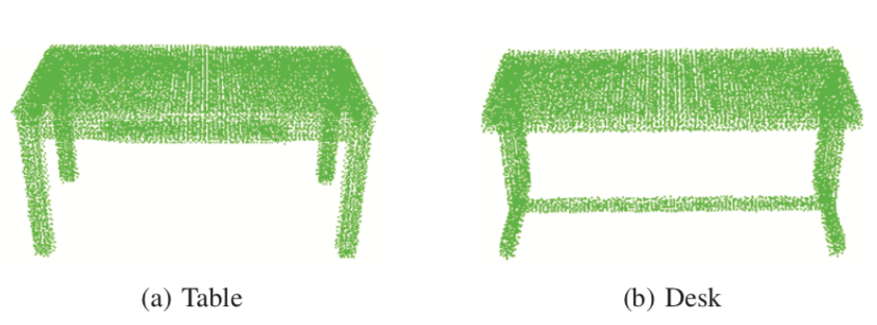
\includegraphics[width=0.65\textwidth]{desk&table.png}
\end{figure}

Suppose there are $K$ classes of objects in the dataset, namely $C_1, \cdots, C_K$. Our aim is to build a classifier that can identify which class each object belongs to. We call $\mathcal{C}$ a probabilistic classifier on $\mathcal{X}$ if it provides an estimate for $\mathbb{P}[x\in C_i\mid x\in \cup\mathcal{X}], C_i \in \mathcal{X}$ for each object $x$, where $\cup\mathcal{X} := \{\cup_{C\in \mathcal{X}} C\}$. For simplicity, we may denote this probability as $\mathbb{P}_\mathcal{C}[x\in C_i]$ when $\mathcal{X}$ is clear from context. 

For any $C \in \mathcal{F} \subset \mathcal{G}$, we have $$\mathbb{P}[x\in C\mid x\in \cup \mathcal{G}] = \mathbb{P}[x\in C\mid x\in\cup \mathcal{F}]\mathbb{P}[x\in \cup\mathcal{F}\mid x\in \cup\mathcal{G}].$$ 

This suggests that we can separate a classifier $\mathcal{C}$ into two stages. Let $\mathcal{F}_1,\cdots, \mathcal{F}_m$ be a partition on $\mathcal{X} = \{C_1,\cdots, C_k\}$. By partition, we mean that $\mathcal{F}_i\cap \mathcal{F}_j = \emptyset, i\neq j$, and $\cup_{i=1}^m F_i = \mathcal{X}$. A classifier $\mathcal{C}$ on $\mathcal{X}$ is mathematically equivalent to a two-stage classifier, where the first stage is a classifier $\mathcal{C}_1$ on $\{\cup\mathcal{F}_1, \cdots, \cup\mathcal{F}_m\}$ and the second stage contains a classifier $\mathcal{C}_{2i}$ for each $\mathcal{F}_i$, defined on $\{C_j: C_j\in \mathcal{F}_i\}$. Although they are mathematically equivalent, breaking up a classifier into two stages may bring potential benefits practically as a classifier is more likely to achieve higher accuracy when the number of classes is reduced. One possible drawback of it, however, is that the increase in the number of classifiers may amplify the total error even though each single classifier achieves better accuracy. In lieu of this trade-off, we need to limit the number of classifiers, and maximize the potential boost in overall accuracy. Therefore, we only apply this two-stage classifier to classes which a one-stage classifier is likely to confuse. For example, the current classifier has a high error rate on table and desk, so we merge these two classes together in the first stage, and leave other classes as they are. In the second stage, we train a classifier that can distinguish table from desk. In this case, the two classifiers are trained independently. 

Without loss of generality, we built a two-stage classifier (Figure \ref{classifier}) based on \textit{PointConv}\cite{pointconv}, which can better distinguish between tables and desks while still achieve comparable accuracy on the other classes of objects. Experiments were carried out using \textit{ModelNet40}\cite{modelnet} to train and test the system.

\begin{figure}[h]
  \caption{Two-stage classifier built on \textit{ModelNet40}.}
  \label{classifier}
  \centering
  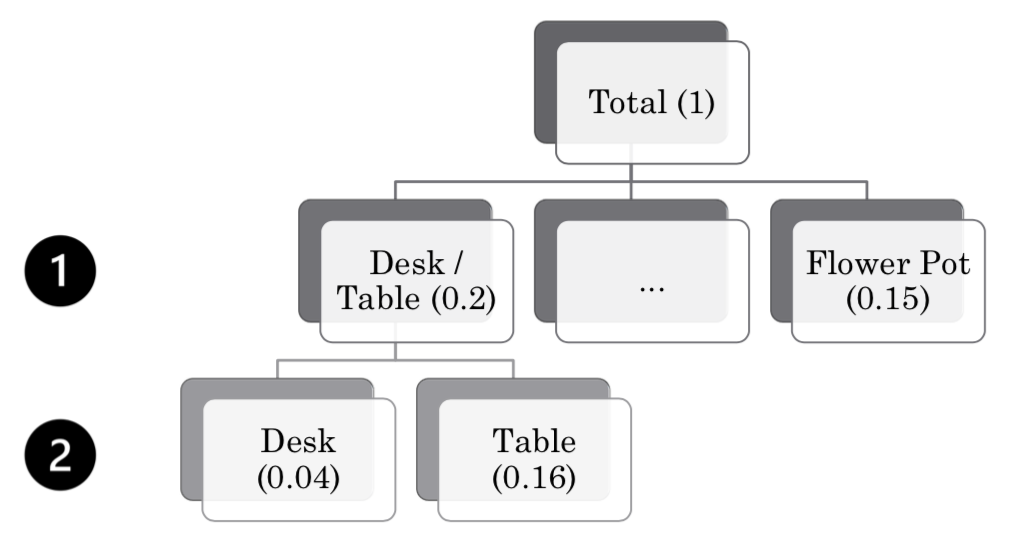
\includegraphics[width=0.65\textwidth]{classifier.png}
\end{figure}

\section{Experimental results}

In order to evaluate the performance of our proposal in terms of accuracy, we conducted experiments on \textit{ModelNet40}. We adjusted the implementation of \textit{PointConv}\cite{pointconv} with PyTorch using the SGD optimizer. 

\textit{ModelNet40} contains 12,311 CAD models from the 40 categories. Unlike \textit{ModelNet10}, the orientation of all the CAD models are not aligned. To alleviate this problem, Wenxuan Wu et al \cite{pointconv} proposed to predict the CAD model from three views. For each CAD model, three views were generated, and the final prediction is based on three predictions generated from the three views. We used the official split with 9,843 CAD models for training and 2,468 for testing.

For a fair comparison, we trained \textit{PointConv} using SGD optimizer and evaluated its performance on the test set. Due to time constraints and limited computing resources, we trained both networks for 40 epochs. The test accuracy of the binary classifier (second-stage classifier) is 88\% and the test accuracy of the first-stage classifier is 92.4\%. 

\begin{table}[!h]
  \centering
  \small
  \caption{Test Accuracy for each class achieved by our method after 40 training epochs using \textit{ModelNet40} dataset (learning rate is 0.001). The values shown in the bracket are the test accuracy achieved by \textit{PointConv} after 40 training epochs (learning rate is 0.001). }
  \label{tbl::acc}
  \begin{tabular}{cccccccc}
    \toprule
    Class & Accuracy & Class & Accuracy & Class & Accuracy & Class & Accuracy \\
    \midrule
    airplane & $1 (1)$ & cup & $\mathbf{0.7} (0.45)$ & laptop & $1 (1)$ & sofa & $1 (1)$\\
    bathtub & $0.92 (\mathbf{0.94})$ & curtain & $\mathbf{0.75} (0.6)$ & mantel & $0.93 (\mathbf{0.95})$ & stairs & $0.9 (0.9)$ \\
    bed & $0.99 (0.99)$ & desk & $\mathbf{0.84} (0.83)$ & monitor & $\mathbf{0.99} (0.98)$ & stool & $0.8 (\mathbf{0.85})$\\
    bench & $\mathbf{0.8}$ $(0.75)$ & door & $\mathbf{0.9} (0.8)$ & night\_stand & $0.80 (\mathbf{0.83})$ & table & $0.88 (\mathbf{0.89})$\\
    bookshelf & $\mathbf{0.97} (0.96)$ & dresser & $\mathbf{0.86} (0.78)$ & person & $0.9 (\mathbf{0.95})$ & tent & $0.9 (\mathbf{0.95})$\\
    bottle & $\mathbf{0.97} (0.94)$ & flower\_pot & $\mathbf{0.15} (0.0)$ &  piano& $\mathbf{0.94} (0.9)$ & toilet & $\mathbf{0.99} (0.98)$\\
    bowl & $0.9 (0.9)$ & glass\_box & $0.9 (\mathbf{0.93})$ & plant & $0.89 (\mathbf{0.92})$ & tv\_stand & $0.9 (0.9)$\\
    car & $\mathbf{0.99} (0.93)$ & guitar & $1 (1)$ & radio & $0.8 (0.8)$ & vase & $0.83 (\mathbf{0.9})$\\
    chair & $\mathbf{0.98} (0.97)$ & keyboard & $1 (1)$ & range\_hood & $0.95 (0.95)$ & wardrobe & $\mathbf{0.7} (0.65)$\\
    cone & $\mathbf{1} (0.9)$ & lamp & $\mathbf{0.85} (0.7)$ & sink & $\mathbf{0.7} (0.65)$ & xbox & $0.7 (0.7)$\\
    \bottomrule
  \end{tabular}
\end{table}

As a result of training our two-stage PointConv with a learning rate of 0.001 during 40 epochs using the \textit{ModelNet40} dataset, it obtained a success rate of \textbf{91.6}\%. With the same learning rate and the same number of iterations, \textit{PointConv} achieved a success rate of 90.6\%. As shown in Tabel \ref{tbl::acc}, the accuracy in many classes has been improved. 

However, while the accuracy in the class Desk has been improved by a bit, the accuracy in the class Table has not been improved. One possible reason is that the accuracy of the binary classifier is only 88\%. Due to time constraints and limited computing resources, we might not select proper hyperparameters for the binary classifier. In addition, it might be helpful to train the two classifiers simultaneously. In this way, we believe the weight functions can be learned more effectively.


\section{Concluding remarks}
In this project, we explored the applications of deep learning methods in 3D geometric data classification. We analyzed the recent breakthroughs to enable deep learning architectures to directly take point clouds as input and found the potential flaw of several state-of-the-art methods that are based on CNN. Then, based on the framework of \textit{PointConv} network and the theory of conditional probability, we proposed a two-stage classifier to specifically address the problem in which CNN is unable to distinguish categories that look alike. By using our method, we have achieved a higher accuracy on the entire dataset.

In future work, we would like to find a proper optimizer so that we can minimize the loss with respect to the two classifiers simultaneously, and aggregate the two classifiers more effectively. In addition, we would like to try different binary classifiers and adopt a more efficient architecture on the second stage classifier to improve the model's performance.

\bibliographystyle{plain}
\bibliography{References}

\end{document}